% Compile with XeLaTeX; original Springer LLNCS class is supplied unchanged.
\documentclass[runningheads]{llncs}
\usepackage[UTF8,fontset=none,scheme=plain]{ctex}
\setCJKmainfont{Noto Serif CJK SC}[BoldFont=Noto Serif CJK SC Bold,ItalicFont=Noto Serif CJK SC,BoldItalicFont=Noto Serif CJK SC Bold]
\setCJKsansfont{Noto Sans CJK SC}[BoldFont=Noto Sans CJK SC Bold]
\setCJKmonofont{Noto Sans Mono CJK SC}
\setmainfont{TeX Gyre Termes}
\setsansfont{TeX Gyre Heros}
\setmonofont{Latin Modern Mono}[Scale=MatchLowercase]
\usepackage{amsmath,amssymb,mathtools,booktabs,array,tabularx,longtable}
\usepackage{graphicx,xcolor,enumitem,placeins}
\usepackage{tikz}
\usetikzlibrary{arrows.meta,positioning,fit}
\usepackage[unicode,colorlinks=true,linkcolor=black,citecolor=black,urlcolor=blue!55!black]{hyperref}
\usepackage{bookmark}
\hypersetup{pdftitle={来源未定的 Release--Acquire 发布网络：候选局部化与精确支持编译},pdfauthor={匿名作者},pdfsubject={中文完整研究稿}}
\renewcommand{\abstractname}{摘要}
\renewcommand{\keywordname}{关键词}
\renewcommand{\figurename}{图}
\renewcommand{\tablename}{表}
\renewcommand{\refname}{参考文献}
\spnewtheorem{cthm}{定理}{\bfseries}{\rmfamily}
\spnewtheorem{clemma}[cthm]{引理}{\bfseries}{\rmfamily}
\spnewtheorem{cprop}[cthm]{命题}{\bfseries}{\rmfamily}
\spnewtheorem{cdef}{定义}{\bfseries}{\rmfamily}
\newenvironment{cproof}{\par\noindent\textbf{证明.}\ }{\hfill$\square$\par}
\newcommand{\RF}{\mathsf{RF}}
\newcommand{\CO}{\mathsf{CO}}
\newcommand{\HB}{\mathsf{HB}}
\newcommand{\FR}{\mathsf{FR}}
\newcommand{\ECO}{\mathsf{ECO}}
\newcommand{\SB}{\mathsf{sb}}
\newcommand{\init}{\mathsf{init}}
\newcommand{\Cov}{\mathop{\mathrm{Cov}}}
\newcommand{\supp}{\mathop{\mathrm{Supp}}}
\newcommand{\Lit}{\mathop{\mathrm{Lit}}}
\newcommand{\ka}{K_{\forall}}
\newcommand{\pv}{P_{\mathrm v}}
\newcommand{\unk}{\textsc{unknown}}
\newcolumntype{Y}{>{\raggedright\arraybackslash}X}
\setlist{nosep,leftmargin=1.6em}
\setlength{\emergencystretch}{2em}
\makeatletter
\let\tableinput\@@input
\makeatother
\graphicspath{{figures/}}
\begin{document}
\raggedbottom
\title{来源未定的 Release--Acquire 发布网络：\\候选局部化与精确支持编译}
\titlerunning{来源未定的 RA 发布网络中的精确支持编译}
\author{匿名作者}
\authorrunning{匿名作者}
\institute{中文完整研究稿}
\maketitle
\begin{abstract}
弱内存执行日志通常只记录读值，不能确定读自哪一次同值写，也不能确定不同线程写入的相对顺序。一次一致性检查虽能给出某个补全，却不能说明每个来源和写序方向是否仍然可能。本文研究固定事件的 Release--Acquire 片段，给出一个面向重复发布网络的候选局部化定理：在完整交替观测、有界阶段密度及有界写覆盖间隔下，来源块可以被锁定而块内身份仍未决；对全部候选来源量化共同前序，可认证跨网络因果分隔，并同时局部化来源边、未决写序与固定写序的覆盖边。所得事件接口界只依赖阶段密度、网络直径、写覆盖间隔和初始化地址数，与阶段总数无关。结合联合关系端口摘要和标准支持编码，该表示保留任意原始来源／写序假设下的全部支持。我们用同值早、晚发布改变写序支持的实例说明身份保留的必要性，并实现不完整来源日志的冲突解释与全部单字段修复。原生 Dat3M 分析对照表明，共同前序规则可以作为已有过滤框架的扩展，新增结论在于明确程序条件所蕴含的整体候选界。实验覆盖双线程交换和多线程有向环；版本载荷的完整诊断任务完成至 32 轮，并对 53 个场景、826 个目标文字进行独立核对。恒定载荷六轮及三线程环四轮的状态超限表明，有界接口并不保证实际编译始终便宜。
\keywords{弱内存 \and Release--Acquire \and 来源分析 \and 知识编译 \and 完整支持 \and 执行日志诊断}
\end{abstract}
\section{引言}
并发程序的一次观测可以遗漏比调度顺序更多的信息。对于同一地址、同一值的多次写，读值不能确定具体来源；对于不同线程的写，线程内程序序不能确定每地址的修改顺序。Release--Acquire（RA）语义进一步允许无法解释为顺序一致交错的观测。因此，分析一段日志时，仅找到一个合法执行，并不足以回答“这个读还可能来自哪些写”或“修改哪一项记录即可消除冲突”。后两类问题需要在既有记录约束下，对原始来源与写序选择求\emph{完整支持}。

一般 RA 一致性问题已经具有复杂的计算边界。最近的结果表明，每地址单写者时可多项式判定，而允许两写者后一般情形仍为 NP-hard~\cite{govind2026}。另一方面，给定 reads-from（RF）关系后判定是否存在合法写序，已有高效算法~\cite{tunc2023}。这两类结果都提示我们：应明确哪些信息已知、哪些选择保留，而不能把“弱内存一致性”视为一个统一的输入合同。本文保留 RF 和 coherence order（CO）两类原始选择，并允许反复添加、撤销针对这些选择的假设。

一个自然路线是将所有合法补全编译为可重复查询的表示。困难出现在编译之前：即使每个实际执行只使用局部的通信边，\emph{全部候选边的并图}也可能很宽。仅从必选 RF 边推导同步，会遗漏所有来源共同保证的因果关系；反过来，将同值发布合并，又会删除诊断所需的来源身份。已有关系分析提供 may/must 上下界和语义过滤接口~\cite{haas2023}，但其一般可靠性结论不会直接给出具体程序族上的候选跨度与接口界。

本文回答以下问题：\emph{在不固定来源身份、不预选 CO 总序的情况下，哪些可检查的发布结构足以保证整个候选表示具有有界接口？该界是否能服务于一个需要完整支持的任务？} 我们考虑有限、完整的阶段观测：每个线程在本轮多次发布相同交替位，随后读取入邻居的上轮位；每轮事件密度和每地址写覆盖间隔有界。多次发布之间可以插入数据写，因此它们的同步效果不同。

主要结论由一条具体推理链组成。首先，完整的交替读序列与单写者标志的 coherence 将来源\emph{块号}锁定为上一轮，却不固定块内来源。其次，块首发布是每个候选来源的共同前序，因而必然先于等待。最后，这些共同前序沿同步网络传播，排除过远 RF、固定远距离 CO，并使固定 CO 的覆盖边也具有有界跨度。后一步需要写覆盖假设；只缩短 RF 或未决 CO 尚不足以约束整个表示。

本文有三项贡献。
\begin{enumerate}
\item 给出来源未定发布网络的局部化定理及完整证明。若网络有向直径为 $d$、每阶段至多 $b$ 个非初始化事件、写覆盖间隔为 $G$、初始化写数为 $a$，则二元选择布局的事件袋大小至多 $(4d+G+3)b+a$，与阶段总数 $n$ 无关。定理约束候选并图，而不是一个已经选定的执行。
\item 将该结构结果接入保持原始标签的联合端口编译，明确二元选择与原子 RF 分组的不同参数界。实例中，旧单例核的候选图包含 $K_{n,n}$，共同来源核则具有统一界；一个身份敏感的 CO 查询说明，不能通过合并同值来源获得这个结果。通用自动机、后缀商和传播编码不作为新的核心贡献。
\item 实现来源日志的全部单字段修复，并提供原生分析对照、不同同步拓扑、独立语义核对和可复现制品。实验的目的在于检验定理能否解释实际候选结构、完整支持是否有用以及编译在何处失效，而非宣称全面优于成熟验证工具。
\end{enumerate}

\section{动机：同值发布并不具有相同支持}\label{sec:motivation}
考虑两个线程交换共享状态的有限内核。线程 A 在一次阶段内先写 $x$，发布标志 $f_a$，再写 $y$，随后再次发布\emph{相同}标志值。线程 B 执行对称操作，并在下一阶段读取 A 的标志。两次发布分别覆盖第一项和两项数据更新；从读到的位值无法判断 B 获得了哪部分同步。这种“分段更新、同值通知”的结构保留了弱同步和竞争写入。

图~\ref{fig:identity} 抽取两轮版本载荷实例中的相关事件。设 $u$ 是 A 第一轮对 $y$ 的写，$a_0,a_1$ 是其早、晚发布，$v$ 是 B 第二轮对 $y$ 的写，$r$ 是 B 的等待，$s$ 是其随后对 $y$ 的读。定义原始文字
\[
 d=\RF(v,s),\quad e=\RF(a_0,r),\quad
 \ell=\RF(a_1,r),\quad q=\CO(u,v).
\]
两个发布都写 1；两位线程在第二轮都对数据写 2，因此数据读的来源身份也未由值唯一决定。

\begin{figure}[tb]
\centering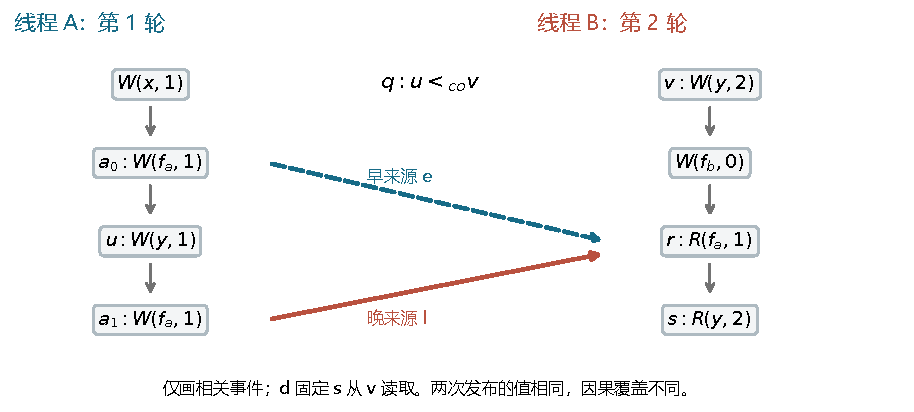
\includegraphics[width=\textwidth]{identity_example.pdf}
\caption{身份敏感的同步。虚线和实线是互斥的 RF 选择，并非同时存在的边；省略的事件仍属于完整输入。}\label{fig:identity}
\end{figure}

在 $\{d,\ell\}$ 下，有
\[
u\;\SB\;a_1\;\RF\;r\;\SB\;s.
\]
由于 $s$ 从 $v$ 读取，write--read coherence 强迫 $u<_{\CO}v$。选择早发布 $a_0$ 时，上述因果链不存在；不仅无法用这条链证明 $q$，实际上 $q$ 的两个方向都有合法补全。表~\ref{tab:motivation} 展示同一个编译结果上的查询、冲突与撤销。附录~\ref{app:witness} 给出允许 $\neg q$ 的完整见证，避免以“未推导出”代替“确有支持”。

\begin{table}[tb]
\caption{同值来源改变 CO 支持。支持是存在合法完整补全，而非静态近似。}\label{tab:motivation}
\centering\begin{tabular}{lll}\toprule
原始假设 $\alpha$ & 一致性 & $q$ 的支持\\\midrule
$\varnothing$ & SAT & 真、假均可\\
$\{d,e\}$ & SAT & 真、假均可\\
$\{d,\ell\}$ & SAT & 仅真\\
$\{d,e,\neg q\}$ & SAT & 仅假\\
$\{d,\ell,\neg q\}$ & UNSAT & 无支持\\
$\{d\}$（撤销来源） & SAT & 真、假均恢复\\\bottomrule
\end{tabular}
\end{table}

这个例子区分了两种知识：$a_0$ 作为块首发布，在任一来源选择下都先于 $r$；但 $u$ 是否先于 $r$ 取决于来源身份。前一种知识适合永久认证和缩小候选表示，后一种相关性必须留在精确查询中。仅保存必选 RF 无法获得前者，合并 $a_0$ 与 $a_1$ 则破坏后者。本文所说的“必要性”是这两个具体不足的反例，不意味着所有正确算法都必须采用本文规则。

\section{语义与完整支持问题}\label{sec:model}
\subsection{固定事件的 RA 片段}
输入由有限事件集合 $E$、线程内程序序 $\SB$、固定地址和固定读写值组成。每个非初始化写都是 release，每个读都是 acquire；每地址有一个初始化写。本文不包含 RMW、fence、SC 操作、非原子访问、动态地址／值或可选事件激活。阶段号属于输入结构，不是执行的全局时间戳，也不要求不同线程的同阶段事件互相同步。

一个完整赋值 $J$ 选择每个读 $r$ 的唯一同址同值来源 $w$，得到 $\RF_J$；并为每地址的写选择严格全序 $\CO_J$，初始化写最小。关系组合 $A;B$ 表示先走 $A$ 再走 $B$，$A^+$、$A^*$ 分别表示传递与自反传递闭包，$A^?$ 为 $A$ 加恒等关系。定义
\begin{align}
 \HB_J &= (\SB\cup\RF_J\cup\init)^+,\label{eq:hb}\\
 \FR_J &= \RF_J^{-1};\CO_J,\qquad
 \ECO_J=(\RF_J\cup\CO_J\cup\FR_J)^+.
\end{align}
其中 $\init$ 将初始化事件置于线程事件之前。合法性要求
\begin{equation}
 \operatorname{irreflexive}(\HB_J;\ECO_J^?).\label{eq:ra}
\end{equation}
它同时要求 HB 无环与四类 WW、WR、RW、RR coherence。本文所有算法、实例与独立核对均使用这个明示片段，不借助不同 RA／RC11 变体之间的语义差异比较性能。将 RF 固定后，CO 仍需满足该公理；将 CO 固定后，RF 也未必合法。

\subsection{原始变量与查询合同}
令 $X$ 包含每个输入 RF 候选的布尔位，以及每个同址无序写对的一个 CO 方向位。方向位的正负分别表示两种次序。预处理证明为常量的位仍属于 $X$，不能从用户接口中删除。合法完整赋值集合记为 $\mathcal V$。

\begin{cdef}[原始支持]
对任意原始文字集合 $\alpha\subseteq\Lit(X)$，定义
\[
 \supp(\alpha)=\{\lambda\in\Lit(X)\mid
       \exists J\in\mathcal V:\ J\models\alpha\cup\{\lambda\}\}.
\]
若不存在满足 $\alpha$ 的 $J$，查询报告 UNSAT；否则返回每个变量两个方向的支持，等价地返回全部必然原始文字。
\end{cdef}

这里的“完整”针对当前假设下的每个原始位，不表示枚举所有完整模型。撤销假设后重新查询同一表示；永久识别不读取 $\alpha$。传播保证仅限于从原始变量假设开始的纯单位传播（UP）。我们不主张任意辅助变量决策或任意外部公式合取之后的全局传播完备。

\subsection{可靠识别核}
识别器保存来源上界 $D(r)$、必选来源 $M$、公共 HB 下界 $H$ 和固定 CO 下界 $L$。不变式是，对任意 $J\in\mathcal V$，真实来源属于 $D(r)$，且 $M\subseteq\RF_J$、$H\subseteq\HB_J$、$L\subseteq\CO_J$。若发现空域、HB 环或固定 CO 环，可靠地拒绝输入。

旧核 $K_0$ 从单例来源得到 $M$，令 $H=(\SB\cup\init\cup M)^+$，由同址写之间的 $H$ 更新 $L$ 并求闭包。若 $H(r,w)$，则 $w$ 不能供 $r$ 读取；若存在同址写 $v$ 使 $L(w,v)$ 且 $H(v,r)$，选择 $w$ 将形成 $r\,\FR\,v\,\HB\,r$，也应删去。对 $L$ 已全序的地址，按同线程读序执行非降来源链过滤，实施 RR coherence。以上步骤迭代到不动点。

新核 $\ka$ 额外保存经认证的公共前序 $B_{\forall}$，将其加入 $H$ 的闭包，并加入规则
\begin{equation}
\frac{D(r)\ne\varnothing\qquad
      \forall w\in D(r):\ u=w\ \lor\ H(u,w)}
     {B_{\forall}(u,r)}.\tag{$R_{\forall}$}\label{eq:cover}
\end{equation}
每次应用只使用此前已经证明的 $H$ 和可靠域；新事实在下一轮参与闭包。$B_{\forall}$ 是 HB 事实，不能伪装为 RF 选择。

\begin{clemma}[来源量化的可靠性]\label{lem:cover}
$R_{\forall}$ 保持上述不变式，且不要求 $D(r)$ 为单例。
\end{clemma}
\begin{cproof}
任取合法 $J$，其唯一来源 $w_J\in D(r)$。规则前提给出 $u=w_J$ 或 $\HB_J(u,w_J)$；接上 $\RF_J(w_J,r)$ 即得 $\HB_J(u,r)$。对推导轮数归纳即可，故不存在循环使用待证结论的问题。
\end{cproof}

规则捕获的关键区别是
\[
 (\SB\cup\bigcap_J\RF_J)^+
 \ \subsetneq\ \bigcap_J(\SB\cup\RF_J)^+
\]
可能成立。例如 $a\,\SB\,b$，读 $r$ 只可能来自同值写 $a,b$；两个 RF 选择都不必然，但 $\HB(a,r)$ 必然。这个规则适合已有 may/must 语义过滤框架~\cite{haas2023}。本文新增的核心证明是接下来从发布条件推出\emph{所有候选}的局部性，而非把该过滤器视作全新的抽象解释框架。

\section{发布网络的候选局部化定理}\label{sec:theorem}
\subsection{可检查的结构条件}
线程构成无自环强连通有向网络 $\mathcal D$，线程数 $p\ge2$，有向直径为 $d$。边 $u\to t$ 表示线程 $t$ 读取 $u$ 的标志。每个非初始化事件有阶段号 $\sigma(e)\in\{1,\ldots,n\}$，线程内阶段依程序序递增。对所有线程给出完整的 $n$ 阶段输入。以下条件定义本文研究的发布网络。

\paragraph{P1：独占标志的重复发布。}
线程 $t$ 独占标志地址 $f_t$，初值 0；数据地址与所有标志地址分离。在阶段 $i$，$t$ 对 $f_t$ 恰有 $m(t,i)\ge2$ 次 release 写，值均为 $i\bmod2$。这些写按 $\SB$ 排列，覆盖该标志的全部非初始化写，没有阶段外隐藏写。发布之间允许固定的数据访问，不要求相邻，也不要求语义上可合并。

\paragraph{P2：完整交替观测。}
线程 $t$ 的阶段 $i$ 在最后一次发布之后，对每条入边 $u\to t$ 各有一次 acquire 读 $r(u,t,i)$，观测 $(i-1)\bmod2$。这些是标志地址的全部读；其来源未预先指定。等待之后仍可有数据访问。这里给出的是完整有限片段，而非缺少未来观测的在线前缀。

\paragraph{P3：阶段密度与写覆盖。}
每阶段所有线程合计至多 $b$ 个非初始化事件。每个数据地址的活动区间是其最早到最晚访问阶段；该区间中的每个完整 $G$ 阶段子区间至少含一次该地址的写，$G\ge1$。标志每阶段有写，自动满足此条件。初始化写数为 $a$。参数 $b,d,G,a$ 可以固定，$n$ 可增长。

条件不预设候选图小宽度，也不要求数据地址单写者。尤其，P3 限制的是写的时间覆盖密度，并不指定不同线程写之间的 CO 顺序。图~\ref{fig:proofchain} 概括各条件在证明中的作用。

\begin{figure}[tb]
\centering
\begin{tikzpicture}[node distance=4mm,box/.style={draw=black!50,rounded corners=2pt,align=center,text width=9.6cm,inner sep=5pt,font=\small},>=Latex]
\node[box,fill=blue!4] (a) {P1、P2：完整交替读链 $\Longrightarrow$ 来源块号锁定，块内身份保留};
\node[box,below=of a] (b) {$R_\forall$ 与网络直径 $d$ $\Longrightarrow$ 共同因果分隔 $h=2d+1$};
\node[box,below=of b] (c) {分隔与写覆盖 $G$ $\Longrightarrow$ RF、未决 CO、$\Cov(L)$ 跨度 $\le\delta$};
\node[box,below=of c,fill=blue!4] (d) {阶段密度 $b$ 与初始化数 $a$ $\Longrightarrow$ 全候选接口 $k=(\delta+1)b+a$};
\draw[->] (a)--(b);\draw[->] (b)--(c);\draw[->] (c)--(d);
\end{tikzpicture}
\caption{核心证明链。$\delta=2h+G$；最后再接精确编译，局部化本身不等于一致性判定。}\label{fig:proofchain}
\end{figure}

\subsection{定理陈述}
记 $N=|E|$，$I$ 为显式输入规模，包含事件、候选和链描述。候选表示仅物化 $D$ 中的 RF、$L$ 未决定的 CO 两向选择、$\Cov(L)$、相邻 $\SB$ 和稀疏初始化边；不把稠密传递闭包 $H,L$ 的每个关系对都物化为边。事件按阶段布局，选择组按最大端点的布局位置排序。组处理时仍可能参与后续组的事件，与本组端点一起组成事件袋。

\begin{cthm}[来源未定发布网络的局部化]\label{thm:main}
对满足 P1--P3 的输入，可靠核 $\ka$ 或证明 UNSAT，或认证下列性质：
\begin{enumerate}[label=(\Alph*)]
\item 每个 $r(u,t,i)$ 的来源域包含于 $u$ 的第 $i-1$ 阶段发布块；$i=1$ 时只含初始化写。若 $i\ge2$，该块的首次发布 $H$-先于 $r(u,t,i)$，即使域仍有多个来源。
\item 令 $h=2d+1$。若非初始化事件 $e,f$ 满足 $\sigma(f)-\sigma(e)\ge h$，则 $H(e,f)$。
\item 令 $\delta=2h+G=4d+2+G$。上述候选表示中所有非初始化边的阶段跨度至多 $\delta$。二元组布局的事件袋大小至多
\begin{equation}
 k=(\delta+1)b+a=(4d+G+3)b+a.\label{eq:k}
\end{equation}
\item 存在保留全部原始 RF／CO 支持的编译图与支持 CNF。置 $S=2^{33k^2+k}$，图节点、边、标签文字及 CNF 文字出现次数均可界为
\begin{equation}
 O(|X|+kNS),\label{eq:size}
\end{equation}
保守构造时间为 $O(I^5+|X|+kNS\operatorname{poly}(k))$。对任意 $\alpha\subseteq\Lit(X)$，支持扫描或支持 CNF 的纯 UP 检出无解，或给出全部必然原始文字。
\end{enumerate}
\end{cthm}

结论 (A)--(C) 是本文的具体语义结构论证；(D) 将其接入第~\ref{sec:compile}节的联合端口构造和标准知识编译接口。大小按表示项数计；序列化标识符时另计 $O(\log I)$ 位。$|X|$ 可以是 $\Theta(N^2)$，所以定理没有声称输出线性、求解器总内存恒定，或常数 $33k^2+k$ 足够小。

\subsection{证明：锁定块号而保留身份}
固定网络边 $u\to t$。标志 $f_u$ 只有一个写线程，因此其 CO 必须等于该线程的发布顺序，初始化在最前。将初始化记为块 0，阶段发布依次记块 $1,\ldots,n$。设 $t$ 的第 $i$ 次等待实际读取块 $q_i$。

RR coherence 使同线程有序读的来源写位置非降。相邻等待的观测位不同，而一个发布块内的值相同，因此 $q_1<\cdots<q_n$。最后一个等待读 $(n-1)\bmod2$，不可能来自值为 $n\bmod2$ 的块 $n$；于是 $q_n\le n-1$。在 $0,\ldots,n-1$ 中放置 $n$ 个严格递增整数，唯一可能是
\begin{equation}
 q_i=i-1\quad(1\le i\le n).\label{eq:block}
\end{equation}

旧核的非降来源链过滤可以得到这一结论：前向贪心计算每个读可接上合法前缀的最小写位置，后向贪心计算可接上后缀的最大位置；域内位于两界之间的候选能分别接上前、后缀。这是单链约束的精确过滤，不意味着该候选已经在全程序中可行。其他可靠规则可继续删域，却不能引入块外来源。剩余域若为空即可拒绝；否则块首发布是所有来源的反身 $H$ 前序，应用引理~\ref{lem:cover} 得到 (A)。来源块内的多个写从未合并。

\subsection{证明：沿网络传播共同因果}
取 $e$ 所在线程到 $f$ 所在线程的一条长为 $\ell\le d$ 的路径。设 $\sigma(e)=i$。阶段 $i$ 的任意事件，包括等待之后的数据操作，都 $\SB$-先于本线程阶段 $i+1$ 的首次发布。由 (A)，该发布先于第一个邻居阶段 $i+2$ 的等待。再沿该邻居程序序到阶段 $i+3$ 的首次发布，即可到第二个邻居阶段 $i+4$ 的等待。

每经过一条网络边推进两阶段，最终到达目标线程阶段 $i+2\ell$ 的等待，再沿程序序到其阶段 $i+2\ell+1$ 的全部事件。因此 $\sigma(f)\ge i+2d+1$ 时必有 $H(e,f)$。所需中间阶段都位于已知输入内；同线程情形直接由程序序得到。这证明 (B)。每跳使用两阶段是由等待在当轮最后发布之后决定的，不能倒走到已经发生的发布；本文不主张 $h$ 是最优界。

\subsection{证明：覆盖所有边种类的跨度}
令来源写 $w$ 位于阶段 $i$，读 $r$ 位于阶段 $j$。
若 $i-j>\delta$，(B) 给出 $H(r,w)$，来源应已删除。若 $j-i>\delta$，考虑长度恰为 $G$ 的整数窗口
\begin{equation}
 [j-h-G+1,\ j-h].\label{eq:pastwindow}
\end{equation}
它位于该地址的活动区间内。P3 给出其中一个同址写 $v$。两侧阶段距离均至少 $h$，故 $H(w,v)$ 和 $H(v,r)$，继而 $L(w,v)$；选择 $w$ 将形成 FR--HB 环。旧核删域规则因此排除这个过老来源。

对未决 CO，只要两个同址写的阶段差至少 $h$，(B) 就已将其方向加入 $L$，所以未决对不可能具有这种跨度。还须单独处理固定 CO 的生成边：若 $u,v$ 位于 $i<j$ 且 $j-i>\delta$，在
\begin{equation}
 [i+h,\ i+h+G-1]\label{eq:coverwindow}
\end{equation}
中由 P3 选同址写 $z$。两侧距离均至少 $h$，因此 $L(u,z)$ 和 $L(z,v)$；$(u,v)$ 不是 $L$ 的覆盖边。此步骤解释了为何写覆盖条件不能只由阶段密度取代。

相邻 $\SB$ 最多跨一阶段，因为每线程每阶段都有发布。初始化事件单独保留至多 $a$ 个；从初始化到各线程首事件的稀疏边足以保留其 HB 闭包。于是所有非初始化候选边跨度至多 $\delta$。

现在按组最大端点排序处理。设本组最大端点位于阶段 $j$。一个较早事件若仍活跃，就还关联某个未处理组。该组的最大端点不早于当前位置，而其跨度不超过 $\delta$，故这个活跃事件不早于阶段 $j-\delta$。尚未引入的未来事件不占当前袋。因此整个袋位于连续 $\delta+1$ 个阶段与初始化集合内，得到式~\eqref{eq:k}。这是实际处理顺序上的存活区间论证，而非只数某一条边的端点。至此证明 (C)；(D) 的构造和计费见下节。

\subsection{条件的边界与同一族上的结构差异}\label{sec:separation}
完整观测不能省略。若有三个发布块 $1,0,1$，却只有两个读观测 $0,1$，它们可以分别来自块 2、3；第一读不必来自初始化。该反例有经独立 RA 定义验证的完整赋值。写覆盖同样有实际作用：保留三线程 16 阶段的标志操作，但只在阶段 1、16 访问数据，则某些数据 $\Cov(L)$ 边跨度为 15。错误代入 $G=1$ 会得到 $\delta=11$；前提检查器拒绝此代入，使用真实覆盖间隔 $G=15$ 后结论成立。

为展示局部化确实改变候选结构，定义双线程族 $P(n,m)$，四个地址 $x,y,f_a,f_b$ 初值为 0，$m\ge2$。阶段 $i$ 令 $z_i=1$、$b_i=i\bmod2$，操作序列为
\begin{align*}
A: &W(x,z_i);\ W(f_a,b_i)_{0};\ W(y,z_i);\\
 &W(f_a,b_i)_{1};\ \cdots;\ W(f_a,b_i)_{m-1};\\
 &R(f_b,b_{i-1});\ R(x,z_i),\\
B: &W(y,z_i);\ W(f_b,b_i)_{0};\ W(x,z_i);\\
 &W(f_b,b_i)_{1};\ \cdots;\ W(f_b,b_i)_{m-1};\\
 &R(f_a,b_{i-1});\ R(y,z_i).
\end{align*}
所有 $W$ 为 release，所有 $R$ 为 acquire。将 $z_i$ 改为 $i$ 得版本载荷族 $\pv(n,m)$。它使数据读仅匹配同轮两位写者，但不区分这两位写者；标志仍只有交替位。版本值需要 $O(\log n)$ 位，所以该变体不保持固定有限的数据值域。

\begin{cprop}[宽度差异与多种支持]\label{prop:separation}
对 $P(n,m)$ 和 $\pv(n,m)$，$K_0$ 的候选图包含 $K_{n,n}$，其最大事件接口随 $n$ 无界。$\ka$ 则满足定理~\ref{thm:main}，其中 $d=1,G=1,b=2(m+4),a=4$，故 $k\le16m+68$。两族至少具有 $4^n m^{2(n-1)}$ 个合法原始赋值；每个非首轮等待的 $m$ 个上轮来源均有合法支持。
\end{cprop}
\begin{cproof}
$K_0$ 锁定标志来源块后，非首轮等待仍有 $m$ 个来源；数据读至少保留本线程本轮与另一线程本轮两个来源。因此除初始化外，不产生跨线程必选 RF。$H$ 没有非初始化跨线程边，$L$ 只固定线程内写序。在地址 $x$ 上，A 的 $n$ 个写与 B 的 $n$ 个写之间 $n^2$ 个 CO 比较全部未决，形成 $K_{n,n}$。任意事件排列中，某一侧第一次全部引入、另一侧尚未全部引入的切口上，已完成侧的 $n$ 个点均有未来邻居，不能退休。局部化界直接由 P1--P3 得到。

对模型数下界，令每个数据读选择本线程本轮的第一项写，等待独立选择任一上轮发布，首轮读初始化。两个数据地址的 CO 均按轮拼接，同轮两位写者的先后各自任选；标志 CO 按程序序。HB 不倒退轮号，跨线程非初始化 HB 至少推进一轮，同轮数据写之间没有跨线程 HB。由此 WW、WR、RW、RR coherence 均成立，详细分类见附录~\ref{app:models}。每轮两个数据地址给出四种独立 CO 选择，非首轮两次等待各有 $m$ 种来源，得到所列下界。
\end{cproof}

该差异仅针对明确定义的 $K_0$ 候选表示；它不是 SAT、BDD、一般 may/must 分析或所有布局编译器的复杂度下界。两族也确实体现弱内存：由 (A)，首轮等待全部读取初始化。对同步边 $u\to t$，任何 SC 全序必须有“$t$ 首次发布 $<$ $t$ 读取 $u$ 初值 $<$ $u$ 首次发布”；沿有向环组合得到矛盾。因此满足 P1、P2 的这些完整观测在 SC 下不可达。上述合法赋值则证明所选数据观测在 RA 下可达。

\section{保持原始支持的精确编译}\label{sec:compile}
局部化提供一个足够小的候选接口，但它尚未回答哪些候选组合合法。本节给出从候选表示到完整支持的构造合同。一般正则关系监视、图消元、选择分组和支持编码已有成熟基础~\cite{kater2023,kucera2021}；本文对这些步骤的使用，必须保证不会丢失前端特意保留的来源身份与 CO 相关性。

\subsection{稀疏生成 CO 与联合关系监视}
令 $g$ 包含 $\Cov(L)$ 和每个未决同址写对所选的一条方向。若 $g$ 无环，则 $g^+$ 恰为扩展 $L$ 的严格全序：有限偏序的覆盖闭包等于自身，而所有未决写对已经选择了一个方向，所以每对写可比；无环性保证严格性。反之，对任意扩展 $L$ 的 CO 总序按其方向选择未决对，得到无环 $g$ 且 $g^+=\CO$。这证明稀疏生成没有预先排除合法写序。已固定的传递比较依然作为原始常量标签存在。

把相邻程序序和初始化生成边记为字母 $s$，RF 记为 $r$，逆 RF 记为 $\bar r$，CO 生成边 $g$ 记为 $c$。式~\eqref{eq:ra} 的禁止闭合游走可用正则语言
\begin{equation}
 \mathcal L=(s\mid r)^+(r\mid c\mid\bar r c^+)^*\label{eq:lang}
\end{equation}
检查。第一段为非空 HB，第二段允许空的 ECO；$c^+$ 实现 CO 闭包，$\bar r c^+$ 实现 FR。该语言有四状态部分 DFA；另用单状态无环监视器检查 $g$。读来源恰一约束由局部计数或原子来源选择实施。每次选择加入\emph{真实}关系边，而不把识别器的所有 $H$ 事实当作已选 RF。

为避免遗忘禁止游走的起点，在 RA 乘积图中为每个事件增加从接受状态回到初态的\emph{标记边}。令普通乘积路径关系为 $R=G^*$，标记边集为 $B_m$，并保存
\[
 T=R;B_m;R.
\]
$T$ 表示恰经过一个标记的路径。原图存在 $\mathcal L$ 闭合游走，当且仅当 $T$ 对角非空：接受路径接一条标记边即闭合，反向将唯一标记旋转到末尾即可。不得对 $T$ 再作传递闭包，因为经过两个标记的环不一定表示一个被禁止的词。

在组 $j$ 处理完后，静态后缀候选集合包含所有剩余替代项可能增加的普通边及尚未加入的标记边。令 $I_j$ 为已出现且仍可能接收后缀边的乘积顶点，$O_j$ 为仍可能发出后缀边的乘积顶点。摘要只保留
\begin{equation}
 \left(R|_{I_j\times O_j},\ T|_{I_j\times O_j}\right),\label{eq:ports}
\end{equation}
并与 CO 监视器、局部度计数组成一个\emph{联合}状态。后缀候选可能互不相容，它们仅决定保留坐标，不能作为实际边加入任何历史。

\begin{clemma}[联合端口的后缀等价]\label{lem:ports}
两个未被拒绝的同层前缀若具有相同联合摘要和计数，则任意相同的后缀选择在二者上同时合法或同时非法。
\end{clemma}
\begin{cproof}
新产生的禁止闭合游走必含后缀新边，否则此前已经拒绝。将游走旋转到一条新边处，并切成新边与历史最大连续片段。每个历史片段从新边目标进入、从新边来源离开，端点必在 $I_j\times O_j$。恰一标记的游走中，至多一个历史片段使用 $T$，其余使用 $R$；若标记来自新边，则所有历史片段均使用 $R$。相同摘要允许在另一历史内替换每段同端点、同标记数路径，得到相同违反；反向同理。这里允许路径重复顶点，符合闭合游走语义。局部恰一条件因计数与剩余组相同而同判。
\end{cproof}

历史片段的替换始终在\emph{同一个}历史内完成。分别合并不同监视器的可达关系，或将互不相容历史的边取并，会失去这个论证。附录~\ref{app:update} 给出闭包更新公式及两个标记不能组合的反例。

\subsection{标签、支持扫描与 UP}
编译器逐组展开选择，用引理~\ref{lem:ports} 合并同层等价摘要，得到有向无环图 $\mathcal G$。每条边携带该组对原始变量的赋值标签；每个原始位沿完整路径恰被赋值一次。被删 RF、单例 RF 和已固定 CO 在根部常量标签中赋值。不同前缀即使合并为同一状态，其入路径标签也保持不同。

逐层归纳可知，接受路径的原始投影恰为 $\mathcal V$。给定 $\alpha$，禁用含相反文字的标签边，分别进行根到节点的前向扫描和节点到接受端的反向扫描。一条未禁用边有支持，当且仅当其来源可从根到达且其目标可到达接受端；汇总这些边的标签得到 $\supp(\alpha)$。不存在接受路径时报告 UNSAT。每次查询成本线性于显式图、标签以及输入／输出长度；撤销假设只需重新扫描。

同一过程可以编码为支持 CNF~\cite{kucera2021}。实现使用其对偶形式：辅助位表示标签被禁用、节点无法前向到达／无法后向接受，以及边已经失去路径支持。原始假设触发相反标签失效；按拓扑序，若所有入边都失效则推出该节点无法前向到达，反向同理。边的标签被禁用、来源不可达或目标不能接受，都足以推出该边失效。对每个原始文字 $\lambda$，加入“含 $\lambda$ 的所有边都失效则 $\neg\lambda$”。UP 因而推出所有无支持文字的否定；若根不能到达接受端，则与根必须可接受的约束冲突。存在合法路径时，将这些辅助位取为其真实失效状态给出满足扩展，故不会产生不可靠推导。这是原始变量的域一致性合同，不是关于任意辅助赋值的更强结论。

\subsection{构造成本与原子 RF 分组}
宽度 $k$ 时，RA 乘积最多有 $4k$ 个活跃顶点，其 $R,T$ 两矩阵合计至多 $32k^2$ 位；CO 普通可达矩阵再用 $k^2$ 位，来源度计数至多 $k$ 个布尔位。联合状态数因而至多 $S=2^{33k^2+k}$。简单候选图有 $O(kN)$ 条边；二元选择组及固定边组数量同阶。每组最多两项，生成图、标签和支持 CNF 得式~\eqref{eq:size}；矩阵更新带来 $\operatorname{poly}(k)$ 因子。

识别阶段中 $D$ 只减，$M,B_\forall,H,L$ 只增，总计至多 $O(N^2)$ 次严格变化。显式矩阵实现每轮保守计 $O(I^3)$，于是粗界 $O(I^5)$ 足够覆盖识别。该界不是精细运行时间预测；保存完整逐条证明轨迹时，轨迹空间需另外计费。至此完成定理~\ref{thm:main}(D) 的证明。

实际实现将一个读的 $t_r=|D(r)|$ 个 RF 二元位合为一个 $t_r$ 路原子组。选择第 $j$ 个来源时，标签同时将该 RF 位置真、其余 $t_r-1$ 位置假。它保留来源身份，只消除了不满足恰一条件的局部组合。

\begin{cprop}[原子分组的保守界]\label{prop:atomic}
定理~\ref{thm:main} 的输入采用原子 RF 组时，令
\[
 k_A=(2\delta+1)b+a,\qquad S_A=2^{33k_A^2+k_A}.
\]
表示大小为 $O(|X|+k_A^2NS_A)$，原始支持合同不变。
\end{cprop}
\begin{cproof}
来源各距读至多 $\delta$，但两个来源之间可能相距 $2\delta$。因此超组跨度应按 $2\delta$ 计；按最大端点排序后的存活窗口给出 $k_A$，不能直接沿用二元界 $k$。每个 $t_r$ 路组有 $t_r$ 个长度 $t_r$ 的标签，标签成本是 $t_r^2$。由 $t_r\le k_A$ 得 $\sum_r t_r^2\le Nk_A^2$；CO 二路组仅需 $O(k_AN)$，按每层状态界复制即得结论。每个合法 RF 恰一赋值与一个组分支一一对应，完整生成边集合相同；非法前缀不会因继续加边而变合法，所以重排选择组不丢合法模型。
\end{cproof}

后处理采用标准的同层、同标签后缀语言商并删除无接受后缀的节点。它减小查询图，但不能降低已经发生的构造峰值。可选 C++ 位集实现执行同一更新代数，产品接口超过 128 位时回退 Python；它不改变摘要等价关系。本文分别报告状态减少、后处理压缩和底层执行成本，避免把它们都归于局部化定理。

\section{完整支持的用途：来源日志诊断}\label{sec:task}
客户端接收一个固定事件、固定读值的输入，以及不完整来源／写序日志 $\alpha$。一个 RF 字段记录某个读的来源身份，一个 CO 字段记录某写对的方向；未记录的字段保持自由。这里“不完整”不表示可以缺少定理所需的阶段事件或等待读值。

对一致日志，客户端返回每个读全部仍可行的来源，以及每个 CO 对仍可行的方向。它们是逐项可能性，不能任意组合为同一个执行。对冲突日志，客户端逐项尝试删除记录，仅在删除后仍 UNSAT 时保留删除，得到\emph{删除意义下极小}的冲突集。这不等于最小基数冲突，也不要求枚举全部冲突。

单字段修复使用完整支持。对每个记录字段 $j$，暂时撤销它；若其余日志仍冲突，修改此字段无法修复。否则查询剩余日志的完整支持：RF 字段返回该读所有有支持的替代来源，CO 字段返回有支持的相反方向。移除原值后，即得到恰好修改一个字段的所有修复。

\begin{cprop}[单字段修复的完备性]\label{prop:repair}
上述过程返回且仅返回能够使整个日志一致的单字段替换。
\end{cprop}
\begin{cproof}
任何修改字段 $j$ 的合法修复都满足撤销 $j$ 后的其余日志，所以新值必在该次支持中。反之，每个返回支持都有满足其余日志和该新值的完整合法见证。遍历全部字段故既不漏修复，也不引入虚假修复。
\end{cproof}

第~\ref{sec:motivation}节的冲突 $\{d,\ell,\neg q\}$ 是删除极小的，并有恰好三种单字段修复：将数据来源从 B 第二轮自身的 $y$ 写改成 A 第二轮的 $y$ 写；将同步来源从 A 第一轮晚发布改成早发布；或将写序方向从 $\neg q$ 改为 $q$。三个选项各有合法见证，它们作为替代建议分别成立，不承诺任意联合使用仍成立。

一次 SAT 调用只能给出其中一个模型，不能用该模型没有选中的来源证明其他来源不可能。SAT 也能实现相同任务，但需要按其查询接口覆盖所有支持。本文同时使用逐原始位完整支持的 SAT 客户端，以及按当前操作只求一致性或相关字段取值的按需 SAT 客户端；两者均返回相同的诊断结果。支持编译的价值在于一次构造后重复使用精确表示，而非将“完整支持”误写成 SAT 无法完成的功能。

实验日志由交换内核生成，覆盖早／晚来源、CO 倒置、冲突及撤销。$n$ 轮任务产生 $8n-7$ 份诊断报告、$20n-19$ 次支持接口调用和 $12n-11$ 个不同假设集合；不使用查询结果缓存。客户端本身不依赖族生成器，可接受任意符合语义输入格式的固定片段。本文尚未用工业部署采集的日志评测，因此将用途定位为可执行的诊断任务，而非部署效果证明。

\section{实验评估}\label{sec:eval}
实验围绕四个问题展开：共同来源推理是否带来实质分析精度变化（RQ1）；完整支持及大规模选定查询是否与独立语义一致（RQ2）；完整诊断任务能增长到何种规模、哪些因素决定成本（RQ3）；改变同步拓扑后，同一定理是否仍能解释候选结构（RQ4）。所有表格来自冻结结果，失败状态与成功记录一并保留。

\subsection{设置、基线与计时口径}
主要输入是第~\ref{sec:separation}节的 $P(n,2)$ 和 $\pv(n,2)$。前者反复写常量 1，后者记录轮次版本。两者有完全相同的同步拓扑和程序序，但版本值排除了跨轮数据 RF；两者的规模结果必须分开解释。它们是可执行研究内核，已有 C11／pthread 和 litmus 导出，未声称从工业库抽取或验证了任意自旋重试。

正式计时在同一 Linux x86\_64 主机上进行，Python 3.10.12，绑定 CPU 0，串行运行。每个配置成功重复三次，报告中位数；第一次资源失败后停止该配置。内存上限 4 GiB，构造时间上限 90 秒，总 wall 上限 240 秒；图预算为 $10^6$ 累计状态、$3\times10^6$ 边。64 轮为单独压力点，仅运行一次，状态／边预算提高为 $2\times10^6/6\times10^6$，其余限制相同。时间包括构造及完整客户端任务，不以单次传播微基准代替总成本。

端口方法包括原子 RF、二元 RF、关闭共同前序规则和关闭原生扩展的消融。SAT 对照使用独立稠密 RA 编码与 Minisat：SAT-full 每次求全部原始支持；SAT-demand 在冲突提取时仅求一致性，修复时只求相关字段全部值，完整快照仍求全部支持。BDD 对照使用 CUDD 后端和 coherence 优先的关系编码，执行同一诊断合同。这些是明示实现的比较，不代表 Dat3M、GenMC 或所有 SAT／BDD 技术的最佳性能。新增 CaDiCaL incidence 编码单独用于正确性核对，不混入这组历史计时。

\subsection{RQ1：与原生关系分析的实质对照}\label{sec:native}
最接近的分析框架是 Haas 等的 may/must 过滤方法~\cite{haas2023}。我们实际调用 Dat3M 4.5.0-alpha 的原生 \texttt{NativeRelationAnalysis}，启用扩展关系分析；提交为 \texttt{b81ec6c55503}（完整摘要见制品）。这是 2026 年实现审计，不是重跑 2023 年论文制品的性能结果。适配器不修改 Dat3M 源码、不重写原生传播器、不调用 SMT 搜索。

两方输入使用相同固定读值 RF 域和相同 RA CAT 公理，并逐事件核对映射；否则，默认分析未获得固定读值会造成不公平的输入差异。四种配置依次提供：仅值域、$K_0$ 事实、$K_0+R_\forall$、以及再补入 HB／CO 闭包和必要删域的完整外部过滤。表~\ref{tab:native} 报告恒定载荷的结果。

\begin{table}[tb]
\caption{原生分析精度审计。关键 HB 是“上轮首次发布到本轮等待”；末列指完整外部过滤与 $\ka$ 的 $H,L,D$ 集合相等。}\label{tab:native}
\centering\small
\begin{tabular}{rrrrcl}\toprule
$n$ & 仅值域 RF & $K_0$ RF & $\ka$ RF & $K_0$ 缺失关键 HB & 完整集合相等\\\midrule
\tableinput tables/native_rows.tex 
\bottomrule\end{tabular}
\end{table}

$K_0$ 输入已提供来源块，但原生输出仍缺少全部关键共同 HB。单独加入 $R_\forall$ 恢复这些边；再执行固定片段的必要闭包与删域，则在 $n=1,2,3,4,8,16$ 全部六项中，与 $\ka$ 的 $H,L,D$ \emph{完整集合}一致。由此得到两个结论：共同来源事实对候选缩减有实质作用；这些事实可接入已有框架，不能把默认实现的缺失解释成框架表达能力不足。定理~\ref{thm:main} 的新义务仍是块锁定、网络传播、覆盖边局部性及参数界。Java 启动成本不用于分析速度比较。

\subsection{RQ2：语义正确性与 32 轮独立核对}
验证分为数学论证、独立实现交叉和完整见证复查。小规模测试枚举原始部分赋值，与不调用识别器的稠密 RA 定义核对；来源、CO 常量、冲突、负 RF 假设与撤销均在原始合同内。正式任务中所有已完成方法和重复运行的完整诊断结果一致；版本载荷至 16 轮有独立稠密 SAT 完整支持对照，BDD 完整对照至 8 轮。表~\ref{tab:validation} 区分各种证据的覆盖范围。

\begin{table}[tb]
\caption{正确性证据及其范围。“选定”不表示穷尽所有假设或所有目标。}\label{tab:validation}
\small\begin{tabularx}{\textwidth}{p{2.5cm}Y Y}\toprule
证据 & 已完成核查 & 能支持的结论\\\midrule
小固定输入 & 新 oracle 的 20 个随机输入全部原始部分赋值，与穷举 RA 一致 & 独立编码的有限语义交叉\\
原有完整任务 & 所有已完成方法与重复结果相同；版本 16 轮 SAT、8 轮 BDD 对照 & 所测诊断查询的全支持一致\\
32 轮选定核对 & 53 场景，826 个目标文字，879 次 SAT 调用；81 个完整见证 & 所选一致性与文字支持一致\\
有向环 & 五个已完成配置逐查询全部原始支持一致；最小环另验纯 UP & 不同拓扑下的实现正确性证据\\
结构核查 & 12 个实例、3,360 个整数窗口及两个前提反例 & 检查具体证书与边界实现\\
干净环境复现 & 50 项测试通过，1 项 CUDD 测试跳过；全部新增实验重跑 & 安装、源码构建与结果可复现\\\bottomrule
\end{tabularx}
\end{table}

32 轮输入含 388 个事件、10,528 个原始位。我们选取阶段 $2,8,16,24,32$，覆盖两线程早／晚来源、倒置 CO、撤销，以及额外负 RF 和否定初始化来源假设，共 53 个场景。新 oracle 使用 CaDiCaL 1.9.5，以实际基本边的右扩展约束表达 HB，独立编码 RF、CO 和 coherence；不调用 $\ka$、端口、布局或 $D/H/L$ 证书。其等价性证明见附录~\ref{app:oracle}。

53 个一致性结果与 826 个正／负目标支持全部相同；41 个场景的完整图答案摘要与旧冻结记录相同，其余为新增查询。可行支持引用 81 个不同完整 RF／CO 赋值，逐一重算 HB／ECO 闭包验证。目标包括条件 CO、同轮两位数据写者、早／晚同步来源、远期排除来源及原始常量。UNSAT 由独立求解器给出，本轮没有生成 DRAT 证明。因此，这些实验增强大规模可信度，但不代替任意 $\alpha$ 下的数学保证。

新编码含 5,131,294 条子句、160,684 个 CNF 变量；原始构造约 13.41 秒，核对阶段约 25.64 秒，后者还包括图查询、见证解码、稠密验证和保存。整个进程峰值 RSS 为 571,800 KiB，允许 8 GiB 内存。它完成的任务与正式完整客户端不同，预算也不同，不能与表~\ref{tab:times} 计算速度比。尤其，旧稠密编码的 32 轮失败不能概括为“SAT 在 32 轮不可行”。

\subsection{RQ3：完整任务增长及机制拆分}
表~\ref{tab:times} 给出版本载荷的完整诊断时间。32 轮原子端口方法完成 249 份报告、621 次支持接口调用，总时间中位数为 16.070 秒。64 轮单次压力点完成 505 份报告和 1,261 次调用，总时间 77.175 秒，峰值 RSS 约 495 MiB；它没有此次独立大规模核对，也不作为重复性能结论。

\begin{table}[tb]
\caption{版本载荷 $\pv(n,2)$ 的完整诊断时间（秒，含构造）。除 $64^*$ 为单次外，成功项为三次中位数。UNK 表示资源超限，ERR 为内存错误报告异常，-- 为未测。}\label{tab:times}
\centering\footnotesize\setlength{\tabcolsep}{3.5pt}
\begin{tabular}{rrr rrrrr}\toprule
$n$ & 事件 & $|X|$ & 端口原子 & 端口二元 & SAT-full & SAT-demand & BDD\\\midrule
\tableinput tables/timing_rows.tex 
\bottomrule\end{tabular}
\end{table}

四轮时 SAT-demand 用时 0.316 秒，快于原子端口的 0.408 秒；八、十六轮时，本组实现中端口完整任务更快。32 轮二元组达到状态预算，稠密 SAT-full 达到 4 GiB 限制，SAT-demand 在内存不足后的错误报告过程又触发异常；BDD 在十六、三十二轮达到 240 秒总时限。所有失败均保留原始状态，不视为 UNSAT，也不以时限替代真实完成时间。图~\ref{fig:times} 只连接已完成点。

\begin{figure}[tb]
\centering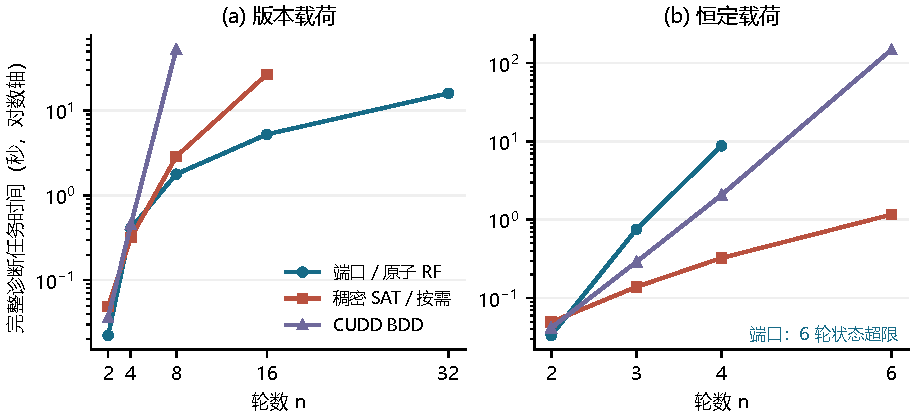
\includegraphics[width=\textwidth]{task_times.pdf}
\caption{同一诊断合同下的总时间。左为版本载荷，右为恒定载荷；缺少数据点表示未完成或未测，具体状态见表。SAT 曲线仅代表该稠密编码的按需实现。}\label{fig:times}
\end{figure}

\begin{table}[tb]
\caption{版本载荷的图规模与任务规模。累计构造状态包含后处理前的状态；后缀商不会消除已发生的构造成本。}\label{tab:size}
\centering\small\setlength{\tabcolsep}{4pt}
\begin{tabular}{r rrr rrr}\toprule
$n$ & 累计状态 & 商后状态 & 最大单层 & 构造秒 & 报告 & 调用\\\midrule
\tableinput tables/size_rows.tex 
\bottomrule\end{tabular}
\end{table}

图~\ref{fig:scaling} 与表~\ref{tab:size} 区分整体规模和每层状态数。版本载荷已测 $n\ge8$ 的最大单层状态数为 1,230；累计状态从八轮 128,666 增长到三十二轮 709,082，商后图从 4,842 增长到 22,554。理论仅保证固定结构参数下的统一上界，不能由这些点推断精确线性运行时间。原始 CO 输出仍随 $n$ 二次增长，客户端解码与报告构造也不可忽略。64 轮中，核心支持查询累计约 15.55 秒，而完整客户端阶段约 42.19 秒。

\begin{figure}[tb]
\centering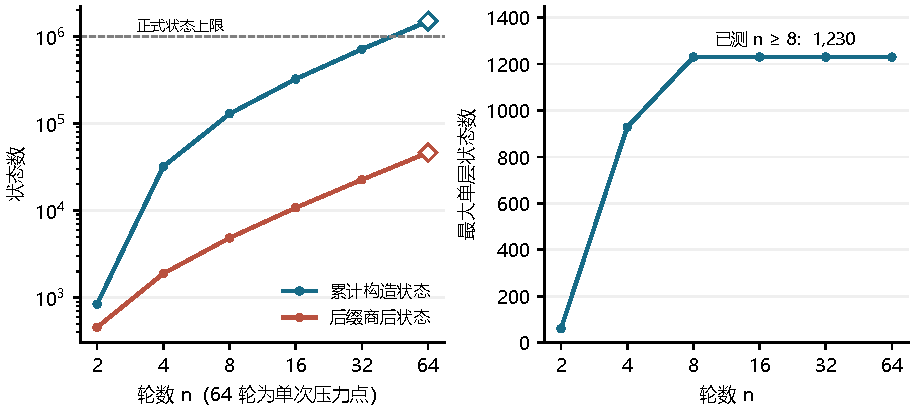
\includegraphics[width=\textwidth]{graph_scaling.pdf}
\caption{版本载荷的构造规模。空心菱形标记提高状态预算后的 64 轮单次点；1,230 是实测单层值，不是一般定理常数。}\label{fig:scaling}
\end{figure}

机制消融给出更明确的因果解释。四轮关闭共同前序，累计状态由 31,930 增为 150,847，完整时间从 0.408 秒增为 2.374 秒；八轮无共同前序达到状态上限。原子 RF 比二元 RF 减少无效局部组合，八轮累计状态从 185,337 减至 128,666。关闭 C++ 后，四／八轮构造从 0.384／1.639 秒变为 2.852／12.615 秒，状态数完全相同；八轮纯 Python 完整任务为 12.758 秒，慢于 SAT-demand。因而实际时间收益同时依赖表示和实现，不能全部归于定理。

恒定载荷给出必要的负面对照（表~\ref{tab:constant}）。四轮原子端口已需 8.783 秒，六轮超过一百万状态；SAT-demand 六轮仍在 1.167 秒完成。恒定载荷允许大量跨轮同值来源，虽仍满足局部化定理，实际状态常数却显著增大。版本载荷的可扩展性部分来自额外观测信息，这不是在相同输入上凭算法消除了困难。

\begin{table}[tb]
\caption{恒定载荷 $P(n,2)$ 的完整任务时间（秒，三次中位数）。}\label{tab:constant}
\centering\begin{tabular}{rrrr}\toprule
$n$ & 端口原子 & SAT-demand & BDD\\\midrule
\tableinput tables/constant_rows.tex 
\bottomrule\end{tabular}
\end{table}

\subsection{RQ4：不同同步拓扑}
为了使结构变化超出双线程加轮数，我们构造有向环上的邻居状态交换。对 $p\ge3$，线程 $t$ 在阶段 $i$ 依次执行
\begin{align*}
 W(x_t,i);\ W(f_t,b_i)_0;\ W(x_{t+1},i);\ W(f_t,b_i)_1;\qquad\\
 R(f_{t-1},b_{i-1});\ R(x_t,i),
\end{align*}
下标按 $p$ 取模。每数据地址有两位写者，每标志只有一位写者。另一个变体让各线程／阶段交替使用两次或三次发布，检查定理不依赖固定块长。这是有实际状态交换含义的有限内核，未冒称某工业协议的完整实现。

三线程时 $d=2,b=18,a=6,G=1$，因此 $h=5,\delta=11,k=222,k_A=420$。因果证据可能经过中间线程，已不同于双线程直接互相同步。图~\ref{fig:ring} 展示结构扫描：十六轮时未决 CO 从 $K_0$ 的 768 对减到 $\ka$ 的 261 对，仍有 45 个多来源等待；八／十六轮实际事件袋大小为 33。故局部化并未把原始不确定性全部固定。

\begin{figure}[tb]
\centering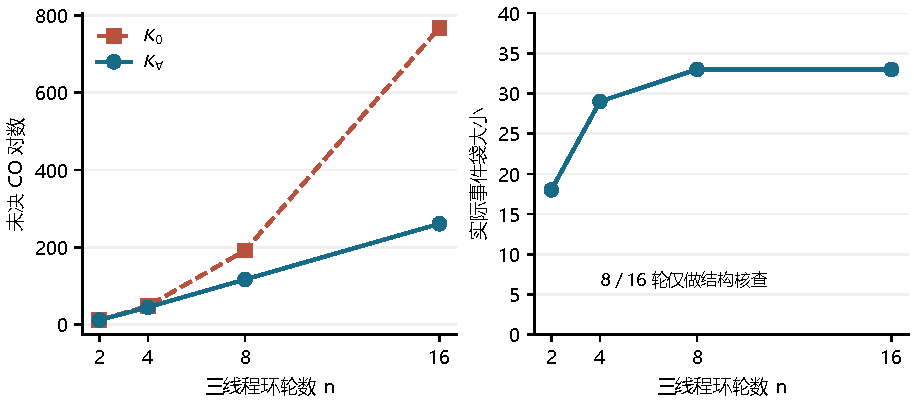
\includegraphics[width=\textwidth]{ring_structure.pdf}
\caption{三线程有向环的结构核查。较大轮数只核查候选与布局，并不表示完成完整支持编译。}\label{fig:ring}
\end{figure}

\begin{table}[tb]
\caption{不同拓扑的单次正确性实验。三线程四轮在累计 1,000,001 状态时停止，未产生一致性答案；其他配置对所有原始位核对完整支持。}\label{tab:ring}
\centering\footnotesize\setlength{\tabcolsep}{3pt}
\begin{tabular}{lrrrrrl}\toprule
配置 & 事件 & $|X|$ & 累计状态 & 商后状态 & 场景 & 状态\\\midrule
\tableinput tables/ring_rows.tex 
\bottomrule\end{tabular}
\end{table}

表~\ref{tab:ring} 中五个完成配置的全原始支持均与独立 CaDiCaL 一致；三线程两轮另验支持 CNF 的纯 UP。所有可行查询均保存完整 RF／CO 见证并重算 RA。最小环的独立 SC 全序编码为 UNSAT，与前述一般论证一致。三线程三轮关闭共同前序后状态数完全相同，此规模上没有额外缩图收益；四轮则在标准预算下失败。这说明同一定理仍解释不同拓扑的候选局部性，但较大的接口足以使实际编译变贵。

\subsection{复现与有效性边界}
制品提供生成器、算法、独立 oracle、查询输入、完整见证、失败记录和逐文件 SHA-256 清单。我们在全新目录与全新虚拟环境中，从源码编译原生扩展并完整复跑新增核查：51 项测试中 50 项通过，1 项因未安装 CUDD 跳过；原完整依赖环境的 51 项全部通过。53 场景／826 支持核对以及全部环配置的状态与图规模均复现。干净环境全流程约 115 秒，此时间是复现回执而非基准性能。

实验不提供工业代表性或普遍速度优势。三次重复仅降低计时偶然性，不能消除构造族选择偏差；图中的中位数不是置信区间。64 轮仅为一次压力点；32 轮独立核对只覆盖选定目标；小实例穷举和测试不等于机器认证的一般证明。强 SAT 编码已经改变 32 轮的可行性，因此论文的主要经验结论是“定理可落地、完整支持可消费、失败可解释”，而非“编译全面胜过 SAT”。
\FloatBarrier

\section{相关工作与贡献边界}\label{sec:related}
\paragraph{关系抽象与 SMT。}
Haas 等~\cite{haas2023} 对内存模型关系建立 may/must 上下界，利用过滤器和外部语义信息简化 SMT 编码。这是本文最接近的分析对象。$R_\forall$ 可以作为其语义过滤器，第~\ref{sec:native}节还给出实际接入结果。因此本文不声称首次发现“不确定来源仍能产生必然 HB”，也不主张新抽象域超越已有框架。区别在于完整交替观测与写覆盖等\emph{具体条件}，以及从这些条件推出全候选 RF、CO 和覆盖边参数界的证明。CAAT~\cite{haas2022} 将广泛公理一致性组合进 SMT 理论求解；本文的固定原始变量支持合同范围更窄，也未解决任意外部公式合取后的传播完备。

\paragraph{自动化内存模型与有界历史。}
Kater~\cite{kater2023} 通过自动机方法自动化弱内存元理论和一致性检查；KATI~\cite{kati2024} 进一步处理带关系交的元理论。本文沿用关系语言及禁止游走的思路，不将自动机、旋转或通用图商视为创新。Ax2Op~\cite{godbole2022} 在明确条件下将公理模型转为有界历史的操作模型。本文已知完整有限事件和候选后缀，处理顺序是编译布局而非未知未来程序执行；其额外义务是保留历史原始身份的条件支持。这是输入和输出合同的区别，不是对整个有界历史框架的严格分离。

\paragraph{RA 一致性与弱内存验证。}
Tunç 等~\cite{tunc2023} 研究给定 RF 后是否存在合法修改序的高效算法。未知 CO 本身并非本文首次处理的问题；本文的 RF 也未知，而且 CO 方向仍供用户假设和查询。Govind 等~\cite{govind2026} 给出单写者可解与两写者困难的边界。本文标志确为单写者，不能把这部分单独当作新可解类；但数据地址有两写者，P1--P3 提供额外结构限制，得到预编译全部支持的参数化结果，不与一般两写者困难性冲突。

基于 potentials 的验证~\cite{bargmann2024} 通过统一语义域和证明规则推理多种内存模型，关注程序断言与演绎证明。本文关注固定观测的来源身份及修改序支持，不替代这种程序级验证。两者都需要准确表达线程从通信中获得什么知识，但其证明对象和输出不同。

\paragraph{逻辑结构与知识编译。}
Conrado 和 Pavlogiannis~\cite{conrado2026} 提出弱内存验证与稳健性的 MSO 框架，以 RF 图表达并抽象修改序，适用的模型范围更广。本文保留原始 CO 查询位，重点证明\emph{选定 RF 之前}的候选并图可被可靠局部化。得到稀疏表示后，MSO／有界树宽方法同样可能适用，故不能声称超出所有结构方法。Kučera 和 Savický~\cite{kucera2021} 系统讨论知识编译到传播编码，并区分原始域一致性与含辅助变量的传播完备。本文采用前一种合同，通用支持编码不构成新的核心定理。

\begin{table}[tb]
\caption{与最近路线逐项对照。表中“本文增加”指本稿需独立完成的证明义务，不声称相应框架无法扩展。}\label{tab:related}
\small\begin{tabularx}{\textwidth}{p{2.4cm}Y Y}\toprule
路线 & 已有假设与输出 & 本文增加的具体义务\\\midrule
关系分析~\cite{haas2023} & 一般 may/must 过滤、保语义 SMT 简化 & P1--P3 蕴含全候选跨度；可接入而非框架分离\\
RF 一致性~\cite{tunc2023} & RF 已定，寻找合法修改序 & RF 仍未定，CO 身份保留，任意假设的全支持\\
单／多写者~\cite{govind2026} & 按每地址写者数划分判定复杂度 & 允许数据两写者，额外周期／密度条件控制接口\\
MSO 结构方法~\cite{conrado2026} & RF 图、逻辑表达、结构验证／稳健性 & 选取 RF 前局部化候选并图，保留 CO 位\\
知识编译~\cite{kucera2021} & 已有编译表示到传播编码 & 前端保证与身份标签使支持合同适用于本片段\\\bottomrule
\end{tabularx}
\end{table}

\section{局限与结论}\label{sec:conclusion}
本文的结构定理依赖明示而较强的程序条件。完整交替观测用于锁定来源块；阶段密度将跨度转为接口；写覆盖约束固定 CO 的生成边。删除这些条件不能沿用现有证明。网络直径和每轮负载若随实例增长，也必须计入参数。语义限定为固定事件 RA，尚不包括动态控制流、RMW、一般屏障或未知未来。将定理扩展到这些范围需要新的推理，而不是直接改换实现选项。

在这些条件内，本文证明了一个可检验的联系：来源身份未决并不妨碍获得共同因果分隔；共同因果分隔又能约束\emph{整个}候选表示，而不是只约束已选执行。身份敏感 CO 查询和完整日志修复说明了为什么公共知识与具体身份必须同时保留。原生分析对照把共同前序规则放回已有过滤框架，核心贡献因此集中在具体条件、参数界及其支持用途。

实验验证了这条联系的可执行性，也显示其实际成本边界。版本交换族能承载 32 轮完整诊断及独立选定支持核对，三线程环改变拓扑后仍满足结构解释；恒定载荷六轮与环四轮的失败则说明结构上有界不等于工程上廉价。后续研究应关注更宽松的观测条件、减少联合状态常数以及真实日志接口。当前结果提供的是一条有证明、有任务、有可复现边界的精确弱内存支持分析路线。

\bibliographystyle{splncs04}
\bibliography{references}
\clearpage
\appendix
\section{见证与模型数下界的细节}
\subsection{身份敏感查询的完整见证}\label{app:witness}
使用第~\ref{sec:separation}节 $P(2,2)$ 或 $\pv(2,2)$ 的事件命名：$A_i:x$ 表示 A 第 $i$ 轮对 $x$ 的写，$i_x$ 为初始化。对于 $\{d,e,\neg q\}$，选择
\begin{align*}
 x:&\quad i_x < B_1:x < B_2:x < A_1:x < A_2:x,\\
 y:&\quad i_y < B_1:y < B_2:y < A_1:y < A_2:y.
\end{align*}
标志 CO 为初始化后按各自程序序排列。全部数据读选择本线程本轮写；首轮等待读初始化，第二轮两次等待都读对方第一轮的早发布。由 $B_2:y<A_1:y$ 得到 $\neg q$。这些边的完整 HB／ECO 闭包通过独立 RA 检查。正向 $q$ 的见证由按轮拼接 CO 的构造给出。因此两个方向确实各有支持，而不是静态近似保留了两个方向。

三种修复的来源候选由恰一 RF 约束解释。固定晚发布与倒置 CO 时，B 第二轮数据读若继续选自身写将违反 WR coherence；改选 A 第二轮同值写可恢复一致。固定自身数据来源与倒置 CO 时，改成早发布解除相应跨线程 HB。固定两项来源时，只剩 CO 正向可行。独立完整支持核对排除了其他单字段替换。

\subsection{按轮见证族的 coherence 分类}\label{app:models}
命题~\ref{prop:separation} 中，数据读取自身本轮写，跨线程 RF 只连接上轮发布与本轮等待。故所有 HB 边不倒退轮号；同轮跨线程 HB 不存在。数据 CO 按轮拼接，每轮两位线程写的次序独立任选。

对同址写 $w\,\HB\,v$，二者若来自不同线程，则必须严格增轮，CO 按轮序一致；同线程则由程序序和轮序一致，满足 WW。对 $w\,\HB\,r$，$r$ 的来源是其线程本轮写；同轮唯一可能 HB-先于 $r$ 的同址数据写就是这个来源，较早轮的写均在其 CO 之前，满足 WR。对 $r\,\HB\,w$，$w$ 必处于更晚轮或同线程后续轮，而来源写在本轮，满足 RW。对 $r\,\HB\,r'$，两个数据读的来源轮次按序增加，满足 RR。

标志写由单线程全序排列。阶段 $i$ 等待选择上轮某次发布，来自该写线程的 HB 前驱不可能晚于所选来源：同阶段更晚发布无法通过另一条不增轮的跨线程路径返回这个等待。其同址 HB 后继写位于后续块。两个 HB 有序等待的来源块不减。因此标志同样满足四类 coherence。初始化最小，且所有基本 HB 边有上述无环分层，故整个执行满足式~\eqref{eq:ra}。同轮 CO 的两向选择和块内来源身份由原始变量区分，模型数量下界成立。

\section{联合端口的增量更新}\label{app:update}
普通关系 $R$ 含恒等路径。插入普通边 $u\to v$ 前，若 $T(v,u)$ 则立即形成恰一标记环，应拒绝。否则使用插入前关系计算
\begin{align}
R'&=R\cup R(*,u)\times R(v,*),\\
T'&=T\cup T(*,u)\times R(v,*)
        \cup R(*,u)\times T(v,*).
\end{align}
可能两次使用新边且在中间经过标记的额外路径，必须含 $T(v,u)$，已在拒绝条件中排除；仅重复普通回路不改变可达性。插入标记边 $u\to v$ 时，若 $R(v,u)$ 则拒绝，否则
\[
 T'=T\cup R(*,u)\times R(v,*),\qquad R'=R.
\]
新标记不能与已有 $T$ 片段连接，否则将错误地允许两个标记。

处理完一组后，投影到新端口 $I_{j+1}\times O_{j+1}$。重新装载矩阵时，只填回已保留关系及普通恒等关系，新端点初始没有其他历史路径。保留项的起点在 $I$、终点在 $O$，任意可组合的两项仍落在同一矩形中；原闭包已包含其组合。引理~\ref{lem:ports} 的路径分解说明，其他删除项以后不会重新变得可观察。CO 无环监视器只需普通 $R$：插边前检查 $R(v,u)$，随后作同样普通更新。

一个最小反例说明标记计数的重要性。普通边为 $0\to3$、$2\to1$，标记边为 $1\to0$、$3\to2$。所有边形成一个含两个标记的环，却不存在恰一标记的闭合游走。若把普通边与标记边混合求闭包，或使用 $T;T$，就会错误拒绝。该反例在实现测试中固定保留。

\section{独立 incidence SAT 编码}\label{app:oracle}
独立 oracle 使用原始 RF、CO 位和附加布尔关系 $H$。对于固定 RF 赋值，令实际基本边 $B=\SB\cup\RF\cup\init$。编码加入
\begin{align}
 B(a,b)&\Rightarrow H(a,b),\\
 H(a,b)\land B(b,c)&\Rightarrow H(a,c),\label{eq:incidence}\\
 \neg H(a,a)&.
\end{align}
RF 基本边使用对应条件文字，固定边条件为真。与对任意中间关系项构造稠密传递约束相比，式~\eqref{eq:incidence} 只沿实际候选基本边右扩展，并流式加入求解器。

\begin{clemma}[oracle 的存在性等价]
配合相同 RF 恰一、CO 全序及 WW／WR／RW／RR 条件，上述编码对原始变量的可满足投影恰为式~\eqref{eq:ra} 的合法赋值。
\end{clemma}
\begin{cproof}
固定 RF 后，按路径长度归纳可得 $B^+\subseteq H$。所有 coherence 限制中 $H$ 都以负极性出现，即“若某 HB 对存在，则相应 CO／RF 条件必须满足”。因此即使满足赋值的 $H$ 含额外事实，把它缩小为 $B^+$ 不会破坏这些限制。对角为假保证 $B^+$ 无环，故得到标准 RA 执行。反之，合法执行取 $H=B^+$ 立即满足基本边、右扩展与 coherence 全部子句。
\end{cproof}

例如 WW 限制要求 $H(w,w')\Rightarrow\CO(w,w')$；WR 要求若 $H(w,r)$ 且 $\RF(v,r)$，则 $w=v$ 或 $\CO(w,v)$；RW 要求若 $H(r,w)$ 且 $\RF(v,r)$，则 $\CO(v,w)$；RR 要求若 $H(r,r')$ 且分别读自 $v,v'$，则 $v=v'$ 或 $\CO(v,v')$。它们均满足上述负极性条件。独立核对不导入 $\ka$ 的任何证书，因此没有用待验证的来源删域帮助 oracle 得出同一答案。

\section{完整结果与制品入口}\label{app:artifact}
论文图表由 \texttt{make\_results.py} 从冻结 JSON 自动生成。\texttt{data/provenance.json} 记录每个输入文件的原路径与 SHA-256；\texttt{data/measurements.csv} 保留成功与失败状态。图表脚本仅整理结果，不重跑算法，不改写原批次。表~\ref{tab:ablation} 补充机制消融，区分累计构造状态和后缀商后的状态。

\begin{table}[ht]
\caption{版本载荷的机制消融。时间为三次中位数（秒）；状态数在重复中相同。}\label{tab:ablation}
\centering\small\begin{tabular}{rlrrrr}\toprule
$n$ & 方法 & 累计状态 & 商后状态 & 构造 & 完整任务\\\midrule
4 & 原子 RF & 31,930 & 1,890 & 0.384 & 0.408\\
4 & 二元 RF & 45,761 & 2,122 & 0.552 & 0.580\\
4 & 无共同前序 & 150,847 & 1,921 & 2.352 & 2.374\\
4 & Python 更新 & 31,930 & 1,890 & 2.852 & 2.875\\
8 & 原子 RF & 128,666 & 4,842 & 1.639 & 1.782\\
8 & 二元 RF & 185,337 & 5,414 & 2.461 & 2.624\\
8 & 无共同前序 & $>10^6$ & -- & -- & UNK\\
8 & Python 更新 & 128,666 & 4,842 & 12.615 & 12.758\\\bottomrule
\end{tabular}
\end{table}

主计时批次有 102 条记录，其中 95 条完成、7 条 UNKNOWN，包含额外预算消融与 64 轮单次项；按需 SAT 批次 25 条，24 条完成、1 条内存错误异常。恒定载荷三轮还保留同一 20 万状态预算下二元组失败、原子组以 43,467 状态完成的对照。正文表取标准预算配置，不以不同预算混算中位数。所有失败详细日志保留在原结果目录。

实验结果的主要对应关系如下：\texttt{support\_task\_20261016} 保存正式完整任务、按需基线与原生分析；\texttt{fm\_evidence\_20261016} 保存 32 轮独立核对、环族、结构审计及干净环境复跑；\texttt{publication\_20261016} 保存较早语义见证与边界记录。每轮构造、查询、完整客户端的中位数分别统计，故不要求分项中位数相加精确等于总中位数。

\subsection{最小复现流程}
自包含证据包为 \texttt{fm\_submission\_20261016.zip}，不含服务器凭据或预编译二进制。解压后在包根目录运行（Linux，Python 3.10+）：
\begin{verbatim}
python -m venv .venv
.venv/bin/python -m pip install -r requirements-fm.txt
.venv/bin/python experiments/fm_reproduce.py --out replay-quick
\end{verbatim}
快速模式验证独立编码、小例、结构条件、整数窗口和前提反例。完整模式需 g++、匹配 CPython 开发头文件及建议至少 8 GiB 可用内存：
\begin{verbatim}
.venv/bin/python experiments/fm_reproduce.py \
    --out replay-full --full
\end{verbatim}
完整模式从源码编译扩展，运行测试、32 轮选定核对和全部六个环配置；三线程四轮的 UNKNOWN 是预期保留结果。输出目录必须为新目录。不同主机的时间和 SAT 见证可以不同，复现比较语义结论、配置状态、图规模与查询数，不要求浮点时间或见证字节完全相同。

逐文件清单、命令、退出码、环境与源码摘要保存在包内 manifest 与复现回执。论文源文件另附图表重建脚本、冻结数据摘录及原始 LNCS 类；使用 XeLaTeX 和 Noto CJK 字体编译。本文数学证明尚未在证明助手中形式化；代码审计、独立 oracle 和干净复跑提供互补证据，不能替代该项形式保证。

\end{document}
